%-----------------------------------------------------
%  Introduction
%-----------------------------------------------------

\section{서론}
\subsection{연구 동기}
Perovskite 구조를 가지고 있는 결정에 레이저를 쏘았을 때 Figure \ref{fig:waveguide} 에서 볼 수 있듯이 빛이 결정의 바깥쪽으로 퍼지는 현상을 관찰할 수 있었고, wave guiding effect에 의한 현상으로 판단하였다. 기존의 perovskite의 구조, 광학적 특성을 분석한 실험에서는 XRD, TRPL, PL등 여러가지 장비를 통해 분석을 하였지만 각각의 장비에 대해서는 깊게 분석하지 못한 면들이 있었다. 특히 PL 분석에서는 PL로 찍었을 때 나오는 개형의 half width과 peak에 대해서만 분석하였기에 exciton peak과 biexciton peak에 대해서 따로 분석해보고자 하였다. 
 
%\begin{figure}[h]
\begin{figure}[t]
	\begin{center}
		\begin{tabular}{cc}
			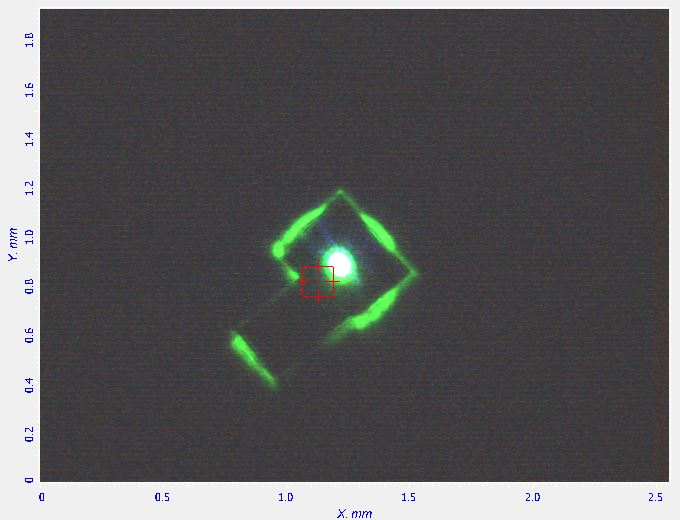
\includegraphics[width=0.7\textwidth]{waveguiding_effect}
		\end{tabular}
	\end{center}
	\caption{만들어진 CsPbBr3 단결정에 레이저를 쏘았을 때 나타나는 모습.}
	\label{fig:waveguide}  
\end{figure}
\subsection{이론적 배경}
\subsubsection{Perovskite}
Perovskite는 L. A. Perovski의 이름을 따서 명명된 물질로, 처음 발견된 CaTiO3  같은 구조를 가진 결정을 통틀어서 부르는 말이다. 일반적으로 ABX3로 쓰며, A와 M에는 여러 금속 양이온들이 해당되고, X에는 보통 16족, 17족 음이온들이 해당된다.Figure \ref{fig:perov} 와 같은 모습이다.

A위치에는 금속뿐만 아니라 유기물인  methylammonium (CH3NH3+)이나 ethylammonium (CH3CH2NH3+)를 넣어 페로브스카이트를 구성할 수 있다. 쇼트키-퀘이서 효율 한계(Shockley Queisser Efficiency Limit)에 의하면 물질의 밴드갭에 따라 전지 효율의 이론적 최댓값이 존재한다. 페로브스카이트는 각 자리에 여러 물질을 바꿔 넣을 수 있으므로 이론적인 최대 효율값에 비슷하게 도달할 수  있는 장점이 있다. 이 뿐만 아니라 가능한 밴드갭 영역이 넓고 꼭짓점을 공유하는 팔면체들의 회로망 덕분에 캐리어의 이동성이 좋아서 전하가 잘 수송되기도 한다.[4] 
또, 페로브스카이트는 합성이 간편하며 태양빛을 잘 흡수하기 때문에 각광받고 있으며, 이와 관련되어 여러 연구가 진행되고 있다. 최근 연구에서는 페로브스카이트에 defect가 존재하여 물성을 탐색할 때 정확하지 못하다는 문제를 해결하기 위해서 단결정을 제작하기도 한다. 본 연구에서는 단결정을 제작하는 새로운 방식 중 하나인 PDMS stamping을 이용하여 단결정을 제작하였다.
\begin{figure}[t]
	\begin{center}
		\begin{tabular}{cc}
			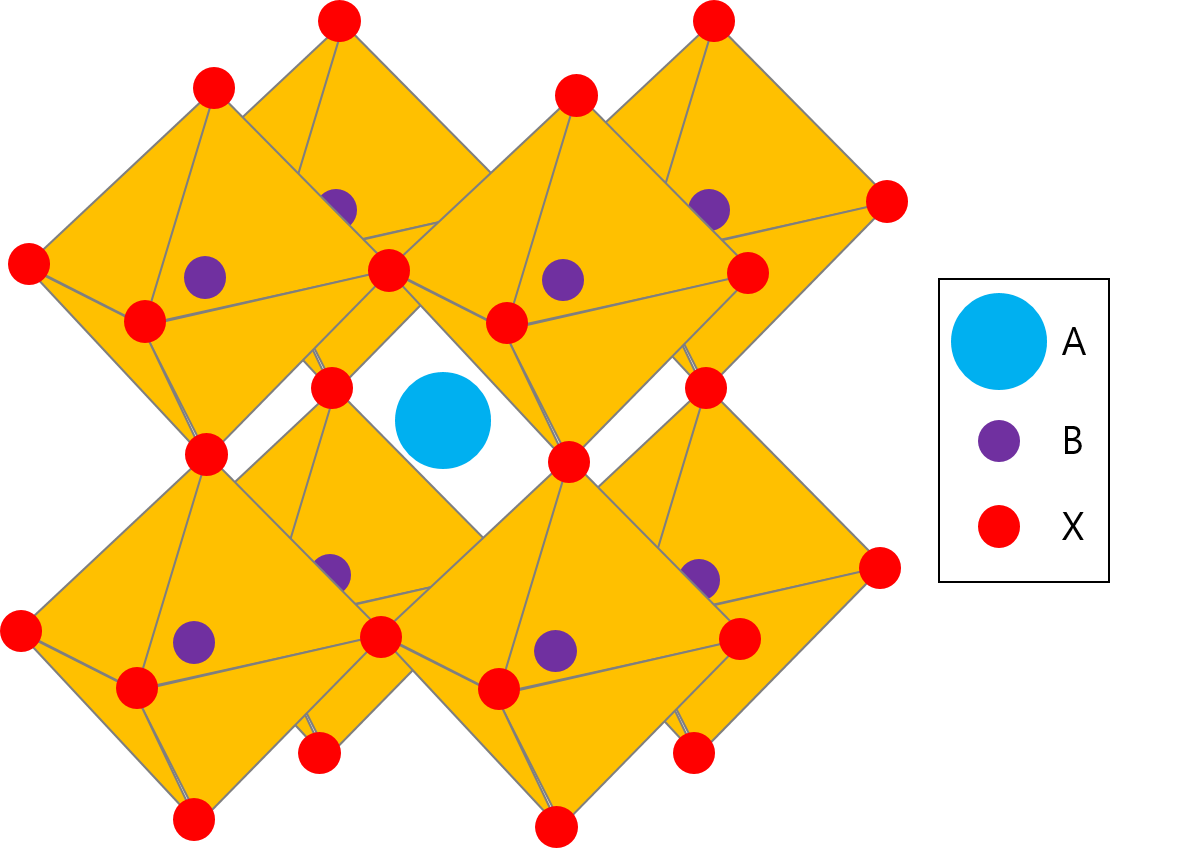
\includegraphics[width=0.7\textwidth]{perovskite}
		\end{tabular}
	\end{center}
	\caption{페로브스카이트의 기본적인 구조를 나타낸 모형.}
	\label{fig:perov} 
\end{figure}
\subsubsection{PL}
PL(Photoluminescence)는 광자를 통해 에너지를 흡수한 물질이 그 에너지를 다시 방출하는 것을 이르는 것이다. 이론적으로는 넣어준 빛의 파장과 동일한 파장의 빛이 나올 수도 있지만 보통은 에너지가 더 낮은, 파장이 더 긴 빛이 방출되게 된다. 

빛이 방출되는 과정은 크게 세 가지로 나뉘는데, photoexcitation, relaxation, radiative recombination 과정으로 나뉜다. photoexcitation은 외부에서 주어진 빛에 의해 전자가 들뜨는 현상을 이르는 것이고 relaxation은 들뜬 전자가 전도띠에서 에너지가 가장 낮은 부분으로, 정공이 원자띠에서 에너지가 가장 높은 부분으로 오는 과정이다. 마지막으로 radiative recombination 과정은 들뜬 전자가 다시 정공과 결합하는 과정을 의미한다. (Figure \ref{fig:pl}를 참고) 이때 방출되는 빛의 파장 별 intensity를 측정하여 PL data 를 얻을 수 있다.
\begin{figure}[t]
	\begin{center}
		\begin{tabular}{cc}
			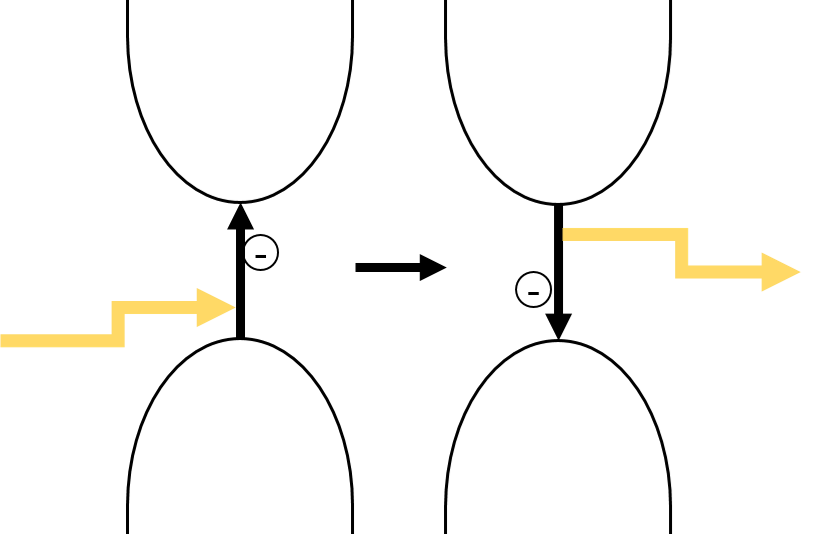
\includegraphics[width=0.45\textwidth]{PL}
		\end{tabular}
	\end{center}
	\caption{들뜬 전자의 relaxation 과정에서 방출되는 에너지.}
	\label{fig:pl} 
\end{figure}
\subsubsection{Exciton, biexciton의 의미}
Exciton은 앞서 말한 PL에서의 측정 과정에서 양공과 전자 하나의 쌍을 말하며, 이 것이 두개가 쌍을 이루고 있을 때 그것을 biexciton이라 칭한다. (Figure \ref{fig:ex} 참고) Triexciton 또한 존재하지만 그 존재 빈도가 극히 적어서 스펙트럼에 나타나지 않는다. 본 연구에서는 PL 분석시에 나타나는 peak의 exciton, biexciton별 분석을 통하여 wave guiding effect의 원인을 분석하는 것이 본 연구의 목적이다.
\begin{figure}[t]
	\begin{center}
		\begin{tabular}{cc}
			
\includegraphics[width=0.8\textwidth]{exciton_biexciton}
		\end{tabular}
	\end{center}
	\caption{exciton 과 biexciton.}
	\label{fig:ex}  
\end{figure}
\subsection{선행연구 및 한계}
이전에 했던 단결정 페로브 스카이트의 구조적 광학적 특성 분석에 관한 연구 에서 XRD와 TRPL, PL을 통하여서 구조적, 광학적 특성을 분석하였다. XRD는 성공적이었으나 위치별로 분석한 PL 분석에서는 스펙트럼이 비대칭적으로 나타났음에도 불구하고 peak와 half width로만 분석했기에 경향성을 분석할 때에 exciton peak 와 biexciton peak의 합의 경향성을 볼 수 있었다. 반면에 exciton 과 biexciton 에 대한 경향성을 따로 볼 수 없었다는 것에 한계가 있다. 본 연구에서는 exciton과 biexciton peak의 intensity를 중점적으로 분석하여서 어떠한 경향성을 가지고 그 원인, 결과는 무엇인지 분석한다.
